\chapter{Testy i bezpieczeństwo systemu}
\label{sec:chapter6}

\section{Testy jednostkowe}

W celu przeciwdziałania błędom, które mogłyby powstać w czasie procesu implementacji aplikacji, kod serwera backendowego został wyposażony w testy jednostkowe, które pozwalają na zweryfikowanie poprawności działania logiki kodu.

Klient frontendowy nie został objęty testami jednostkowymi, gdyż oceniono, że nakład pracy wymagany do pokrycia frontendu testami byłby nieproporcjonalny do korzyści, które zostałyby w ten sposób osiągnięte. Poprawność działania serwera backendowego jest kluczowa z punktu widzenia stabilności aplikacji. Klient frontendowy w zdecydowanej większości operacji nie wykonuje istotnych obliczeń, a jedynie deleguje je do backendu, więc pokrywanie części frontendowej testami nie zostało uznane za konieczne.

Testy jednostkowe są uruchamiane na dwa sposoby, w sposób manualny oraz automatycznie przy użyciu narzędzia ciągłej integracji GitHub Actions. Mechanizm ciągłej integracji zostanie omówiony w Rozdziale \ref{chapter:ci}.

W sposób manualny, testy jednostkowe można uruchomić przy użyciu narzędzia Maven, wywołując w katalogu projektu backendowego polecenie \verb|./mvnw test| \cite{maven_guide}. Przykładowy wynik takiego testu przedstawiono na Rysunku \ref{fig:carbon_ut}. Wydruk wygenerowany przez narzędzie zawiera informację o liczbie sukcesów, błędów oraz pominiętych testów.

Struktura kodu źródłowego testów jednostkowych została zorganizowana w następujący sposób: każda pokryta testami klasa ma w repozytorium bliźniaczą klasę z przyrostkiem \verb|Test|. Dla przykładu, klasa \verb|ImageIOConverter| (odpowiadająca za konwersję plików graficznych) posiada odpowiadającą klasę \verb|ImageIOConverterTest|, zawierającą testy jednostkowe metod publicznych wspomnianej klasy.

Na rysunku \ref{list:carbon_example_ut_code} przedstawiono przykładowy kod źródłowy testujący metodę \verb|convertTo| klasy \verb|ImageIOConverter|. 

Metoda \verb|test_convertTo_webpToPng|, jak sugeruje nazwa, weryfikuje poprawność konwersji obrazów z formatu webp na format png. W niniejszej klasie testowej zostały również zdefiniowane podobne metody dla formatów png oraz jpg, jednakże nie zostały one przedstawione w niniejszym dokumencie w celu zachowania czytelności zapisu.

Metoda testująca została oznaczona adnotacją \verb|@Test| pochodzącą z biblioteki JUnit. Dzięki temu oprogramowanie uruchamiające testy może w zautomatyzowany sposób ustalić, które metody należy potraktować jako metody testujące \cite{junit_user_guide}.

W ciele metody \verb|test_convertTo_webpToPng| znaleźć można przykładowe wywołanie testowanej metody \verb|convertTo| (linia 36). Do metody przekazano ścieżkę pliku wejściowego, ścieżkę pod którą ma zostać zapisany plik wejściowy, a także format docelowy, czyli png.

W linii 38 wykonywana jest asercja przy użyciu obiektu \verb|mimeTypeDetector| oraz funkcji \verb|assertThat| dostarczanej przez bibliotekę AssertJ.

Obiekt \verb|mimeTypeDetector| klasy \verb|ApacheTikaMimeTypeDetector| wykrywa rodzaj pliku na podstawie odczytu sygnatury pliku. Funkcja \verb|assertThat| pozwala upewnić się, że wartość zwrócona przez obiekt \verb|mimeTypeDetector| jest równa wartości oczekiwanej. Jeśli wartości będą się różniły, zostanie rzucony wyjątek, a test zostanie oznaczony jako nieprawidłowy. \cite{assertj_docs}

\begin{figure}[h]
    \centering
    \setlength{\fboxsep}{0pt}
    \setlength{\fboxrule}{0.4pt}
    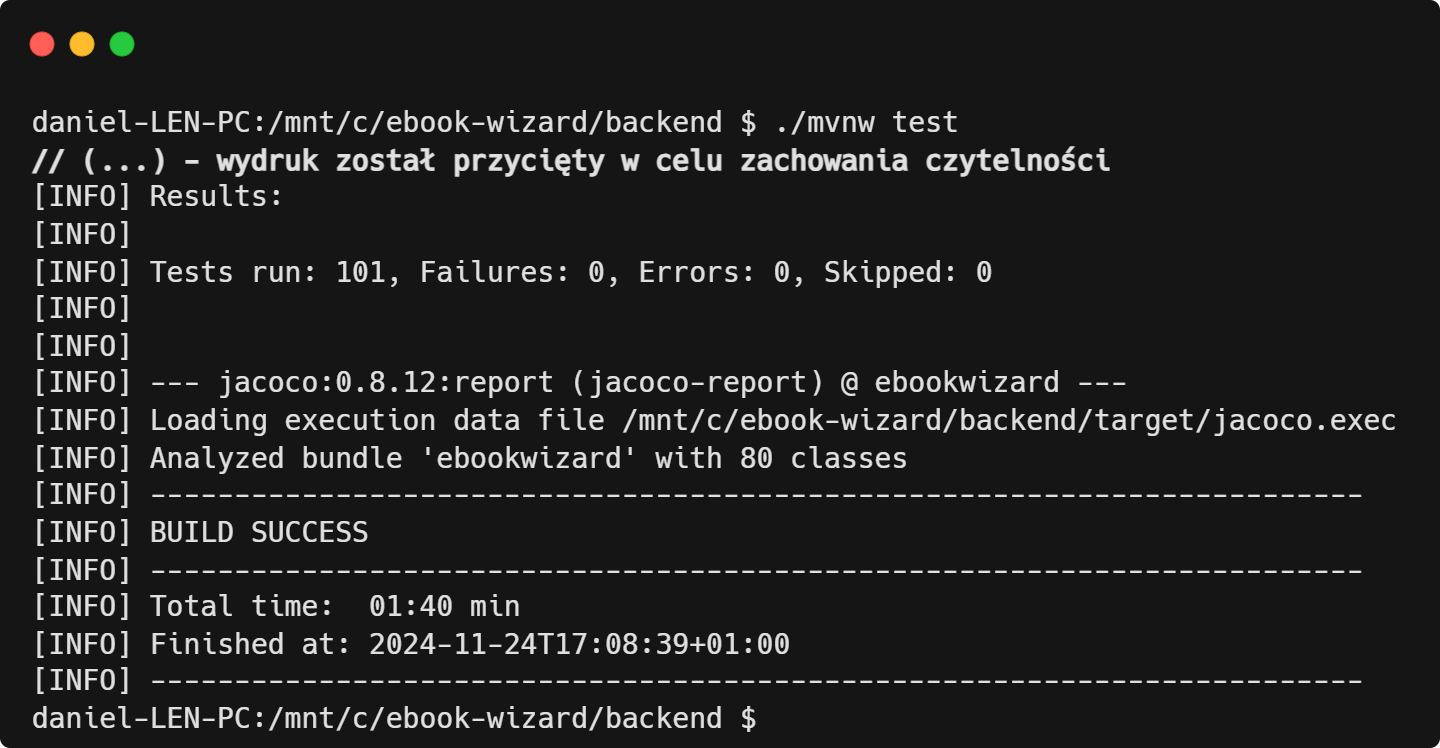
\includegraphics[width=0.69\textwidth]{chap6/carbon_ut.png}
    \caption{Przykładowy fragment wyniku wywołania testów jednostkowych}
    \label{fig:carbon_ut}
\end{figure}

\begin{figure}[h]
    \centering
    \setlength{\fboxsep}{0pt}
    \setlength{\fboxrule}{0.4pt}
    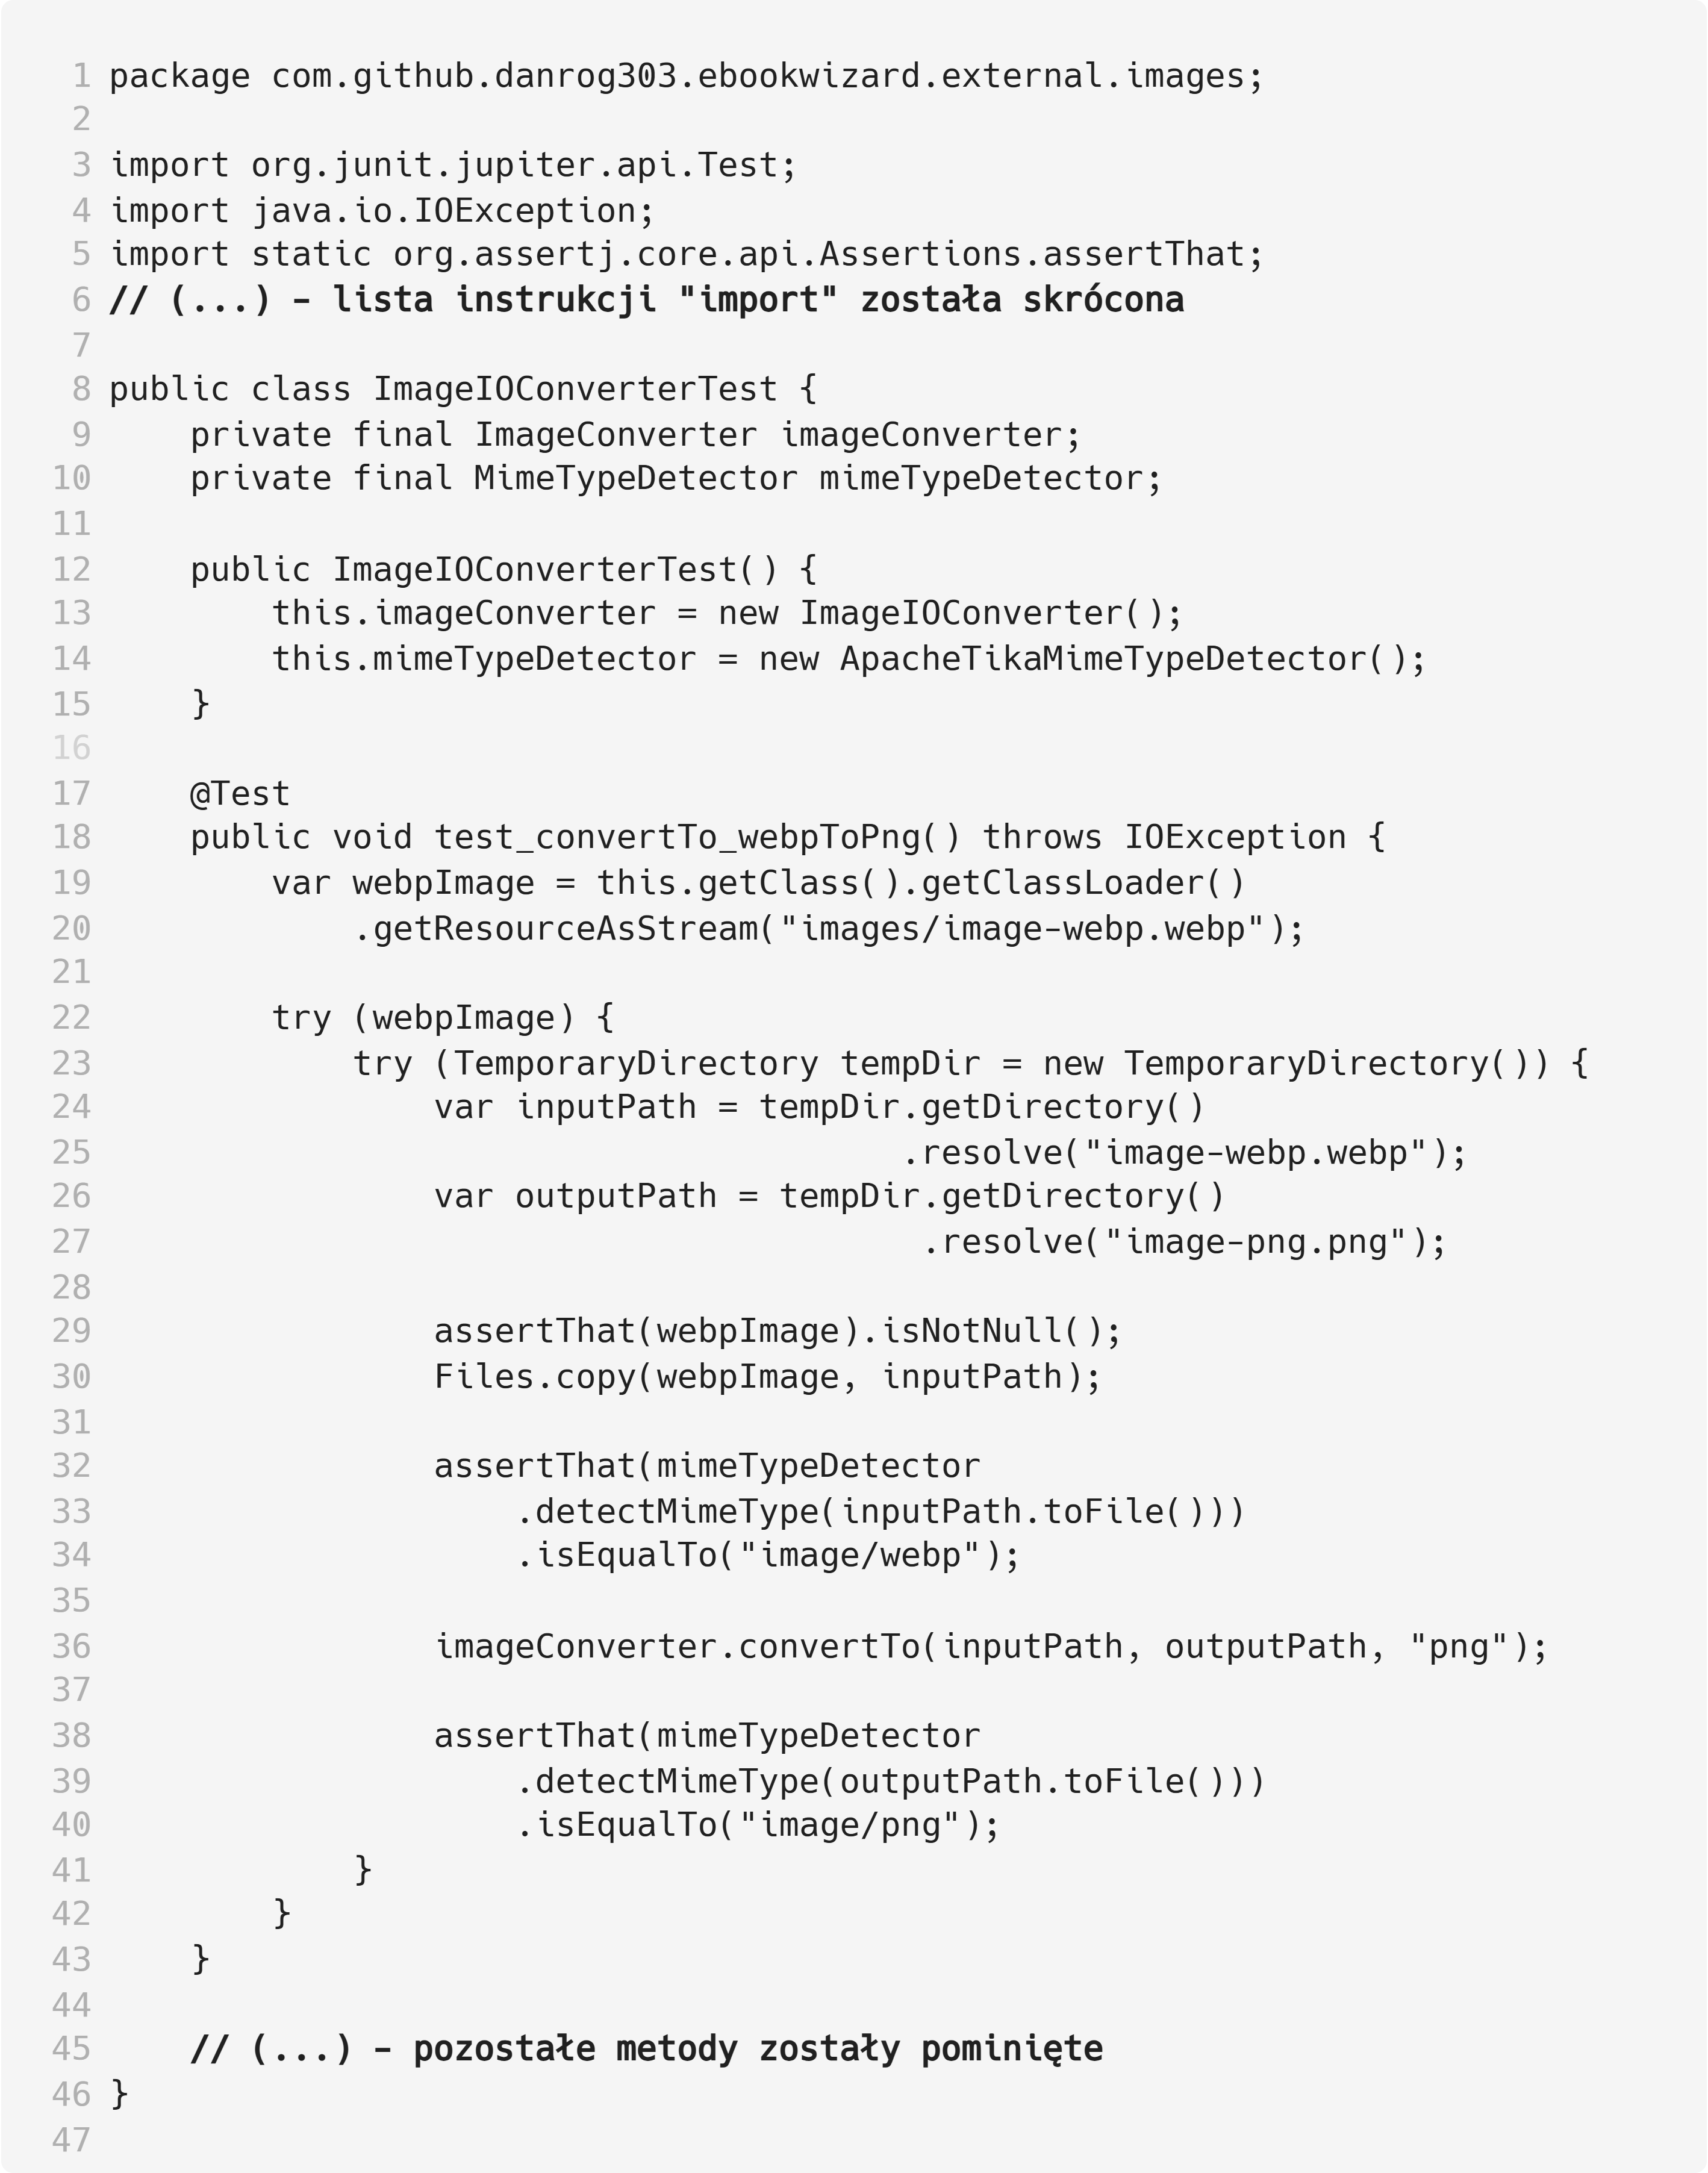
\includegraphics[width=0.9\textwidth]{chap6/carbon_example_ut_code.png}
    \caption{Przykładowy kod źródłowy metody testującej}
    \label{list:carbon_example_ut_code}
\end{figure}


\section{Ciągła integracja}
\label{chapter:ci}

Aby uniknąć omyłkowego przesłania do repozytorium GitHub kodu zawierającego błędy, wykorzystany został mechanizm ciągłej integracji.

Jak podaje literatura, ciągłą integracją nazywamy proces automatycznego przeprowadzania kompilacji i testowania oprogramowania za każdym razem, gdy nowa wersja programu zostanie zewidencjonowana w systemie kontroli wersji. \cite{ci_book}

Jako dostawcę mechanizmu ciągłej integracji wybrana została usługa GitHub Actions. Wybór został podyktowany tym, że GitHub Actions posiada natywną integrację z serwisem GitHub, który przechowuje pełną kopię kodu źródłowego aplikacji. Ponadto, GitHub Actions oferuje darmowy plan użytkowania, który pozwala użytkownikom prywatnym na wykonywanie automatyzacji bez ponoszenia opłat. \cite{github_actions_docs} Kolejną zaletą, która odróżnia GitHub Actions na przykład od konkurencyjnego oprogramowania Jenkins, jest brak konieczności utrzymywania własnego serwera. GitHub Actions w domyślnej konfiguracji wykorzystuje serwery GitHuba, co znacząco upraszcza proces konfigurowania usługi ciągłej integracji. \cite{github_actions_docs, jenkins_docs} 

W systemie GitHub Actions, konfiguracja ciągłej integracji odbywa się przy pomocy plików z rozszerzeniem yaml. Pliki te muszą znajdować się w katalogu \verb|.github/workflows| w repozytorium i muszą mieć zawartość zgodną z dokumentacją usługi. Szablon dostarczany przez GitHub Actions określa kiedy dany skrypt ma zostać uruchomiony (na przykład: gdy pojawia się nowa wersja kodu źródłowego), na jakim systemie operacyjnym ma zostać wywołany skrypt, a także jakie kroki mają zostać wykonane. \cite{github_actions_docs}

W repozytorium Ebook-Wizard, procesowi ciągłej integracji poddawany jest zarówno kod serwera frontendowego, jak i kod serwera backendowego. Na Rysunku \ref{listing:carbon_example_ci} został przedstawiony plik yaml stanowiący konfigurację ciągłej integracji dla repozytorium Ebook-Wizard. 

W kodzie tym zdefiniowane są dwie akcje, wykonywane równolegle w momencie przesłania nowej wersji kodu do repozytorium. Obie akcje są uruchamiane na systemie Ubuntu (linia 10 i 51 listingu \ref{listing:carbon_example_ci}). 

Pierwsza z akcji, nazwana \verb|build_backend|, zajmuje się zbudowaniem i przetestowaniem backendu. Najpierw w linii 12 pobierany jest kod źródłowy projektu. Następnie, w liniach 13-18 pobierane jest środowisko uruchomieniowe Java. W liniach 19-30 pobierane są niezbędne zależności systemowe (Pandoc oraz Calibre). Następnie, w linii 32-35 konfigurowany jest dostęp do repozytorium GitHub Packages. Finalnie, w liniach 36-38 wywołane jest polecenie \verb|mvn clean verify|, które pobiera zależności aplikacji, wykonuje kompilację, a następnie uruchomienie testów jednostkowych.

\begin{figure}[h]
    \centering
    \setlength{\fboxsep}{0pt}
    \setlength{\fboxrule}{0.4pt}
    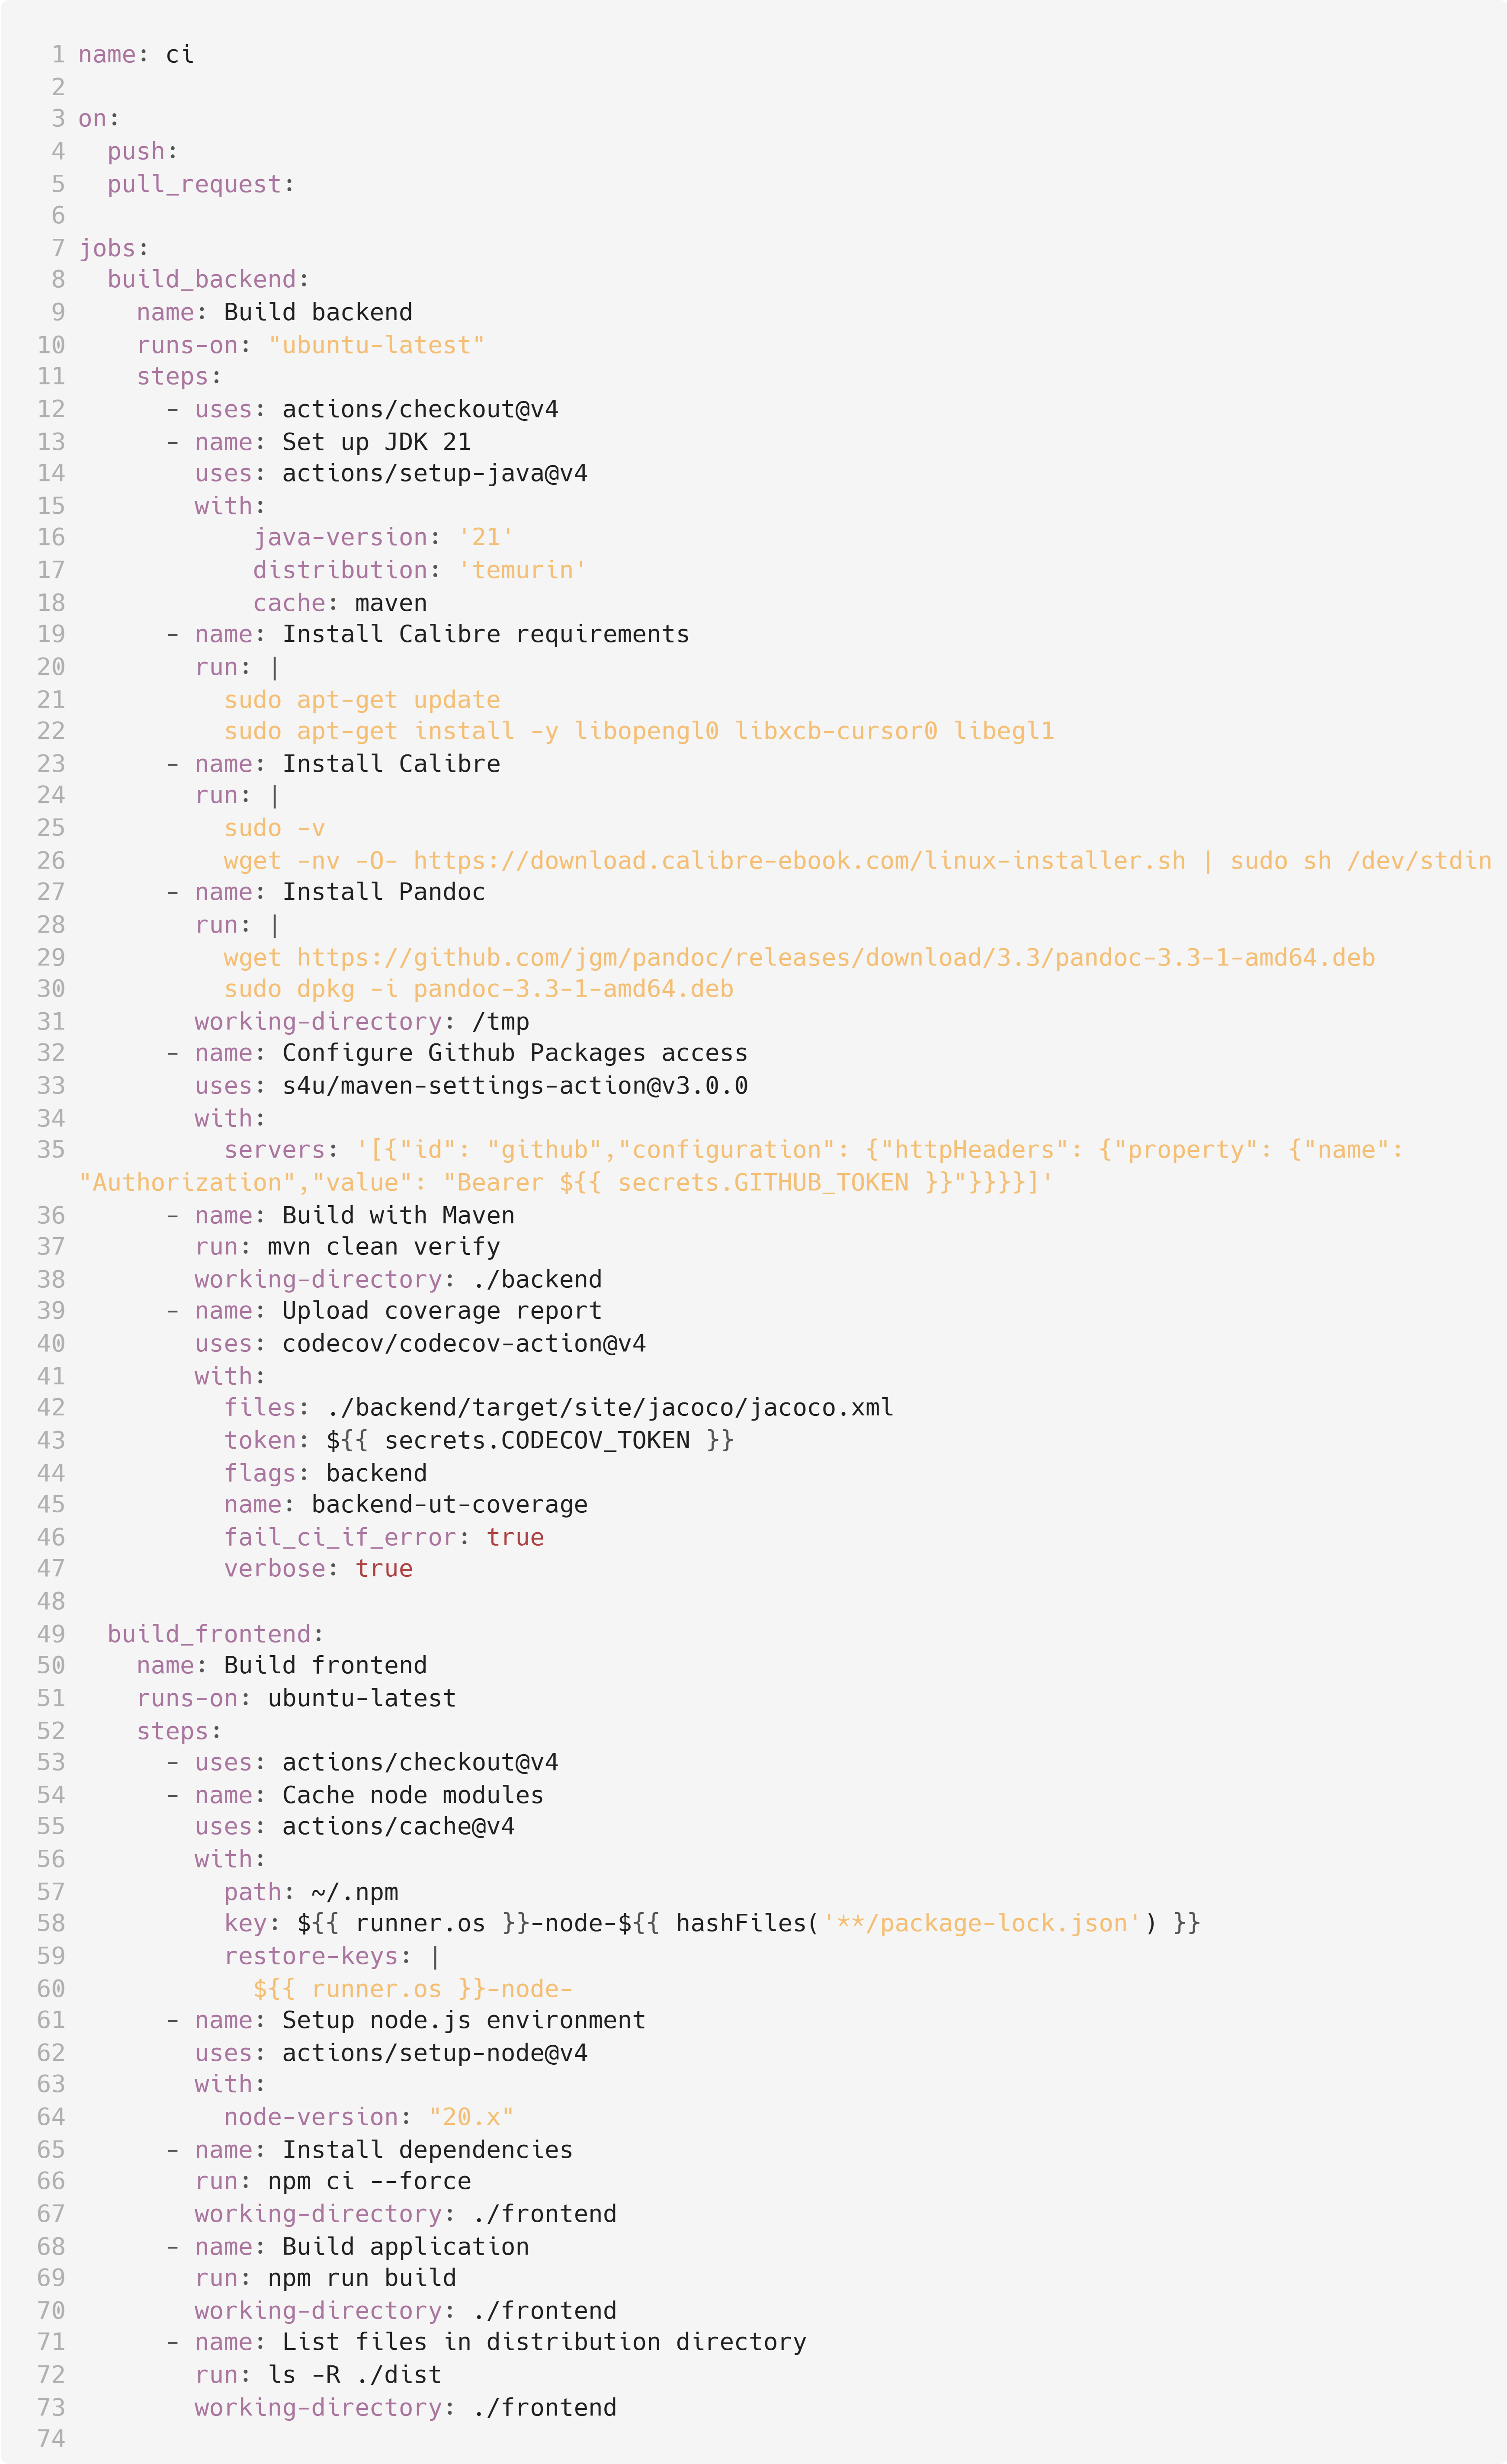
\includegraphics[width=0.88\textwidth]{chap6/carbon_example_ci.png}
    \caption{Konfiguracja ciągłej integracji frontendu i backendu}
    \label{listing:carbon_example_ci}
\end{figure}

Akcja \verb|build_frontend|, jak sugeruje nazwa, weryfikuje czy frontend buduje się poprawnie. Najpierw w linii 53 ponownie pobierany jest kod źródłowy z repozytorium. Następnie, w linii 54-60 wykonana jest próba przywrócenia bibliotek z cache, co skraca czas wywołania skryptu. Konfiguracja środowiska uruchomieniowego NodeJS odbywa się w liniach 61-64, a w liniach 65-67 pobierane są zależności programowe. Finalny proces budowania odbywa się w liniach 68-70. Jeśli budowanie się nie powiedzie (np. wystąpił błąd w kodzie źródłowym), wówczas proces npm zakończy się z niezerowym kodem wyjścia, a GitHub Actions wyświetli błąd. W celu ułatwienia debugowania, w liniach 71-73 dodano wyświetlanie zawartości folderu z artefaktami kompilacji.

\section{Bezpieczeństwo i stabilność}

W procesie implementowania serwisu Ebook-Wizard został podjęty szereg kroków, które mają za zadanie zapewnić użytkownikom możliwie najwyższe standardy bezpieczeństwa i stabilności. Najistotniejsze z tych kroków zostały zebrane i opisane w poniższych podrozdziałach.

\subsection{Konfiguracja zapory sieciowej na poziomie dostawcy usług}

Serwer, na którym pracują procesy frontendowe oraz backendowe, został zabezpieczony poprzez wykorzystanie zapory sieciowej.

Korzystając z panelu serwisu hostingowego, na którym uruchomiony jest frontend i backend, skonfigurowana została zapora sieciowa, która blokuje każdy niedozwolony ruch przychodzący. Jedyne publiczne w Internecie porty to port 443 (w celu zezwolenia na komunikację HTTPS) oraz port 80 (w celu ustanowienia przekierowania dla użytkowników, którzy spróbują połączyć się z serwerem przy użyciu protokołu HTTP). 

Dodatkowo, aby umożliwić zdalną konfigurację maszyny, został otwarty port 22, czyli port usługi SSH. Usługa SSH pozwala nawiązać zdalną sesję terminala przy użyciu standardowej powłoki systemu Linux. \cite{linux_administration_cookbook} Dostęp do tego portu jest filtrowany na podstawie adresu IP. Wyłącznie autoryzowane adresy mogą wykonać próbę połączenia do serwera SSH.

\subsection{Wykorzystanie szyfrowania SSL}

Dostęp do obu serwerów Ebook-Wizard (serwera frontendowego i backendowego) odbywa się za pośrednictwem bezpiecznego protokołu HTTPS. Dostawcą certyfikatu jest firma Let's Encrypt, która udostępnia darmowe certyfikaty SSL dla właścicieli witryn internetowych. \cite{lets_encrypt_docs}

Dzięki wykorzystaniu protokołu HTTPS, dane przesyłane pomiędzy klientem a serwerem są szyfrowane, co uniemożliwia podejrzenie transmisji przez osoby trzecie. Ponadto, protokół HTTPS gwarantuje że połączenie odbywa się z autentycznym serwerem, co eliminuje ryzyko podszywania się pod serwer. \cite{https_http_in_action}

Konfiguracja certyfikatów SSL na serwerze Ebook-Wizard odbywa się za pośrednictwem oprogramowania nginx. Proces nginx nasłuchuje połączeń na porcie~443 (domyślny port protokołu HTTPS), a następnie przekierowuje żądanie użytkownika do frontendu lub backendu. Ponadto, nginx dba o to, aby ustanowić automatyczne przekierowanie z protokołu HTTP. Jeśli użytkownik w pasku kontrolnym przeglądarki ręcznie odwoła się do adresu \verb|http://|, serwer nginx automatycznie przekieruje go do witryny z przedstrostkiem \verb|https://|.

Na listingu \ref{listing:carbon_nginx} przedstawiono fragment pliku \verb|nginx.conf|, który przedstawia konfigurację protokołu SSL. W linii 15 zdefiniowane jest, że serwer ma używać SSL i nasłuchiwać na porcie 443. W liniach od 16 do 19 zdefiniowana jest konfiguracja certyfikatów SSL. Dodatkowo, w liniach od 22 do 30 zdefiniowano konfigurację przekierowania z protokołu HTTPS na HTTP. Aby umożliwić działanie tego przekierowania, w 
 linii 27 serwer został skonfigurowany do nasłuchiwania na porcie 80 (domyślny port HTTP). \cite{packt_nginx, https_http_in_action}

\begin{figure}[h]
    \centering
    \setlength{\fboxsep}{0pt}
    \setlength{\fboxrule}{0.4pt}
    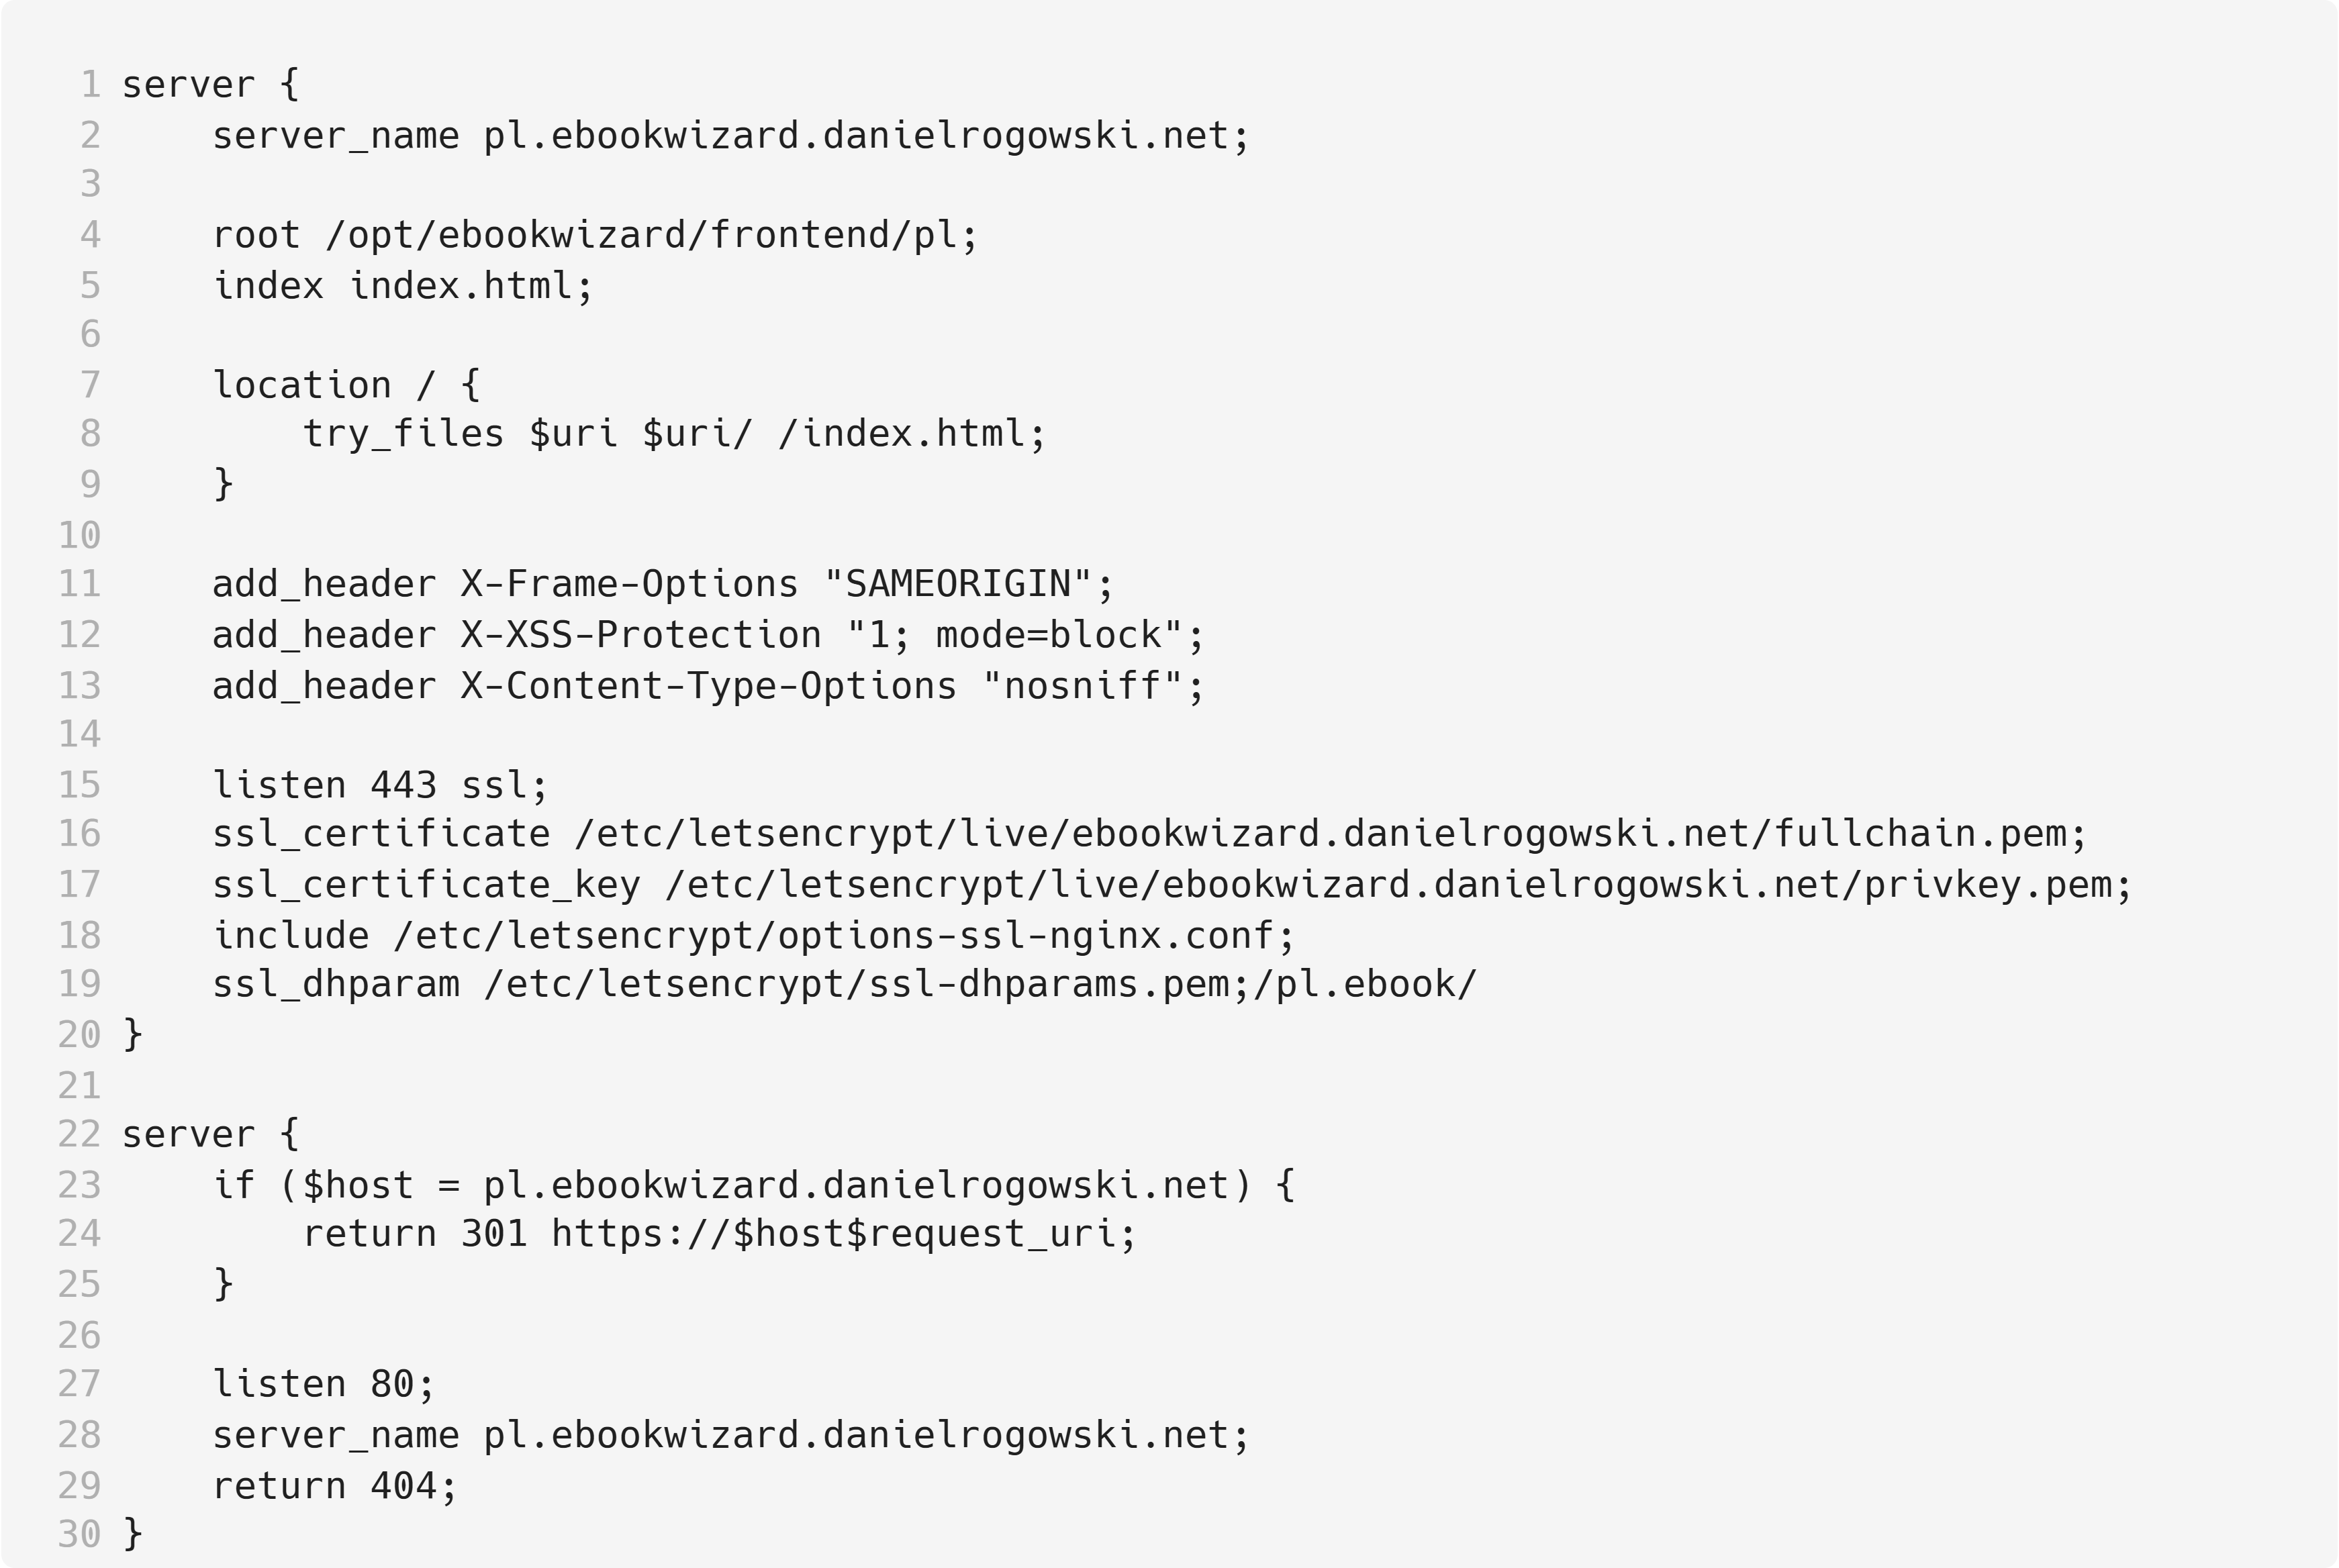
\includegraphics[width=0.88\textwidth]{chap6/carbon_nginx.png}
    \caption{Fragment konfiguracji oprogramowania nginx}
    \label{listing:carbon_nginx}
\end{figure}

\subsection{Wykorzystanie usług sprawdzonych dostawców}

Kluczowe usługi serwisu Ebook-Wizard, takie jak uwierzytelnianie oraz przechowywanie plików, zostały powierzone zewnętrznemu operatorowi, firmie AWS (\textit{Amazon Web Services}). Za uwierzytelnianie odpowiada usługa Amazon Cognito, natomiast pliki przechowywane są w usłudze Amazon S3. Usługi firmy Amazon napędzają również mechanizm kolejkowania zadań (Amazon Simple Queue Service), system generowania głosu (Amazon Polly) oraz wysyłanie e-maili (Amazon Simple E-mail Service).

Jak podaje strona operatora Amazon, usługi AWS posiadają szereg certyfikatów, takich jak ISO 27001, ISO 27017 oraz ISO 27018. Usługi AWS przechodzą również regularne audyty.~\cite{aws_compliance} Usługi AWS wykorzystywane są przez firmy takie jak Bank Pocztowy, linie lotnicze LOT i koncern Ringier Axel Springer (właściciel m. in. platformy Onet). \cite{aws_case_Studies} Fakt, że AWS używany jest nawet przez banki, udowadnia, że jest to operator gwarantujący najwyższe standardy bezpieczeństwa.

\subsection{Wykonanie audytu narzędziem SonarQube}

W celu zapewnienia możliwie jak najwyższego poziomu bezpieczeństwa i stabilności aplikacji, projekt frontendowy oraz projekt backendowy zostały przeskanowane przy użyciu narzędzia statycznej analizy kodu SonarQube. Statyczna analiza kodu to zautomatyzowana analiza kodu źródłowego bez jego wykonania, pozwalająca na wyszukiwanie luk w zabezpieczeniach, błędów w kodzie oraz problemów ze stylem kodu. \cite{sonarqube}

W początkowych etapach rozwoju projektu, SonarQube wykrył stosunkowo dużo problemów, które zostały następnie załatane. Na Rysunku \ref{fig:sonarqube} przedstawiono porównanie raportów wygenerowanych przez SonarQube w dniu 22 października 2024 r. (dzień wykonania pierwszego audytu) oraz w dniu 8 grudnia 2024 r. (dzień finalizacji prac nad kodem źródłowym aplikacji). Jak zaprezentowano na wspomnianym raporcie, w końcowej fazie implementacji aplikacji SonarQube nie znalazł żadnych problemów z bezpieczeństwem (Security), niezawodnością (Reliability) ani utrzymaniem kodu (Maintainability).

\begin{figure}[h]
    \centering
    \setlength{\fboxsep}{0pt}
    \setlength{\fboxrule}{0.4pt}
    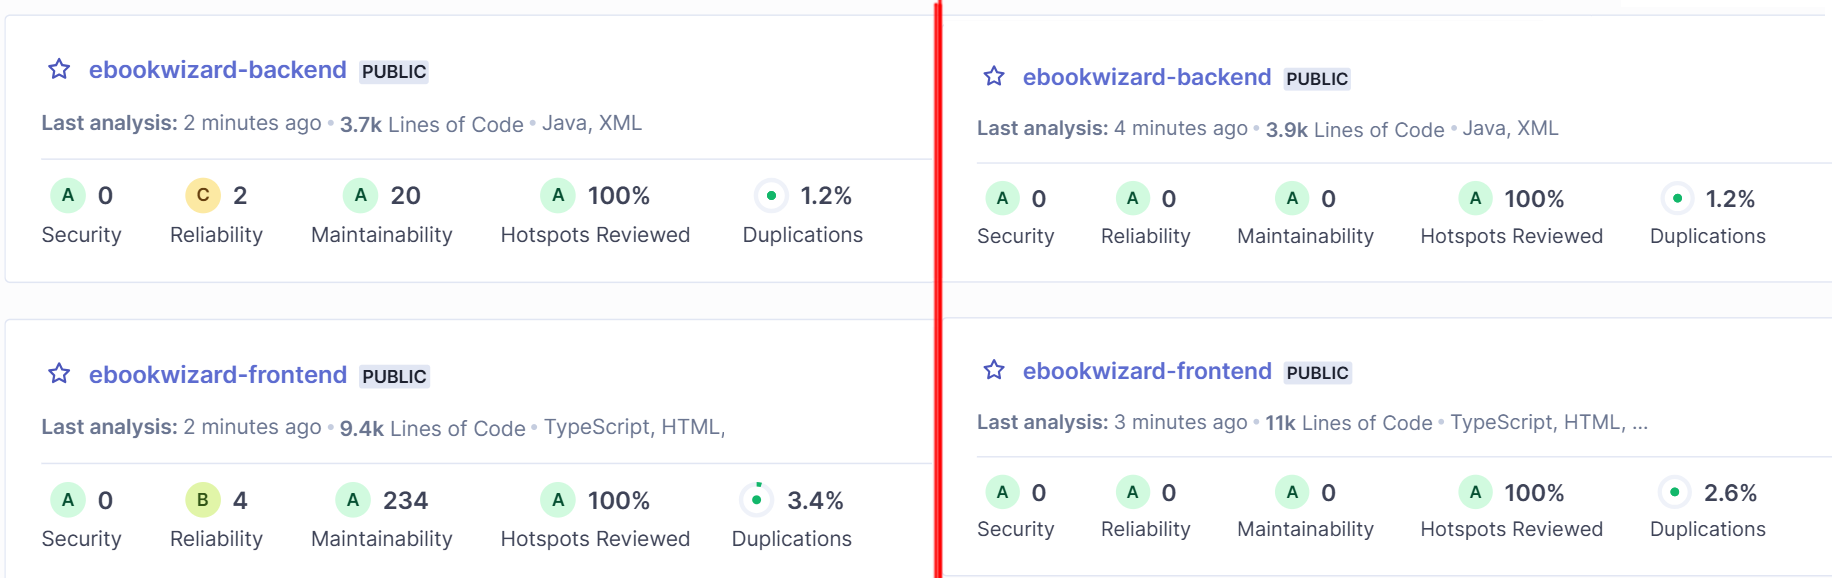
\includegraphics[width=0.88\textwidth]{chap6/sonarqube.png}
    \caption{Wynik przeprowadzenia audytu narzędziem SonarQube (porównanie)}
    \label{fig:sonarqube}
\end{figure}